\pdfoutput=1
\documentclass[a4paper,pdflatex,ja=standard]{bxjsarticle}

% ---Setting about the geometry of the document----
% \usepackage{a4wide}
% \pagestyle{empty}

% ---Physics and Math Packages---
\usepackage{amssymb,amsfonts,amsthm,mathtools}
\usepackage{physics,braket,bm}

% ---underline---
\usepackage{ulem}

% --- sorround the texts or equations
% \usepackage{fancybox,ascmac}

% ---settings of theorem environment---
% \usepackage{amsthm}
% \theoremstyle{definition}

% ---settings of proof environment---
% \renewcommand{\proofname}{\textbf{証明}}
% \renewcommand{\qedsymbol}{$\blacksquare$}

% ---Ignore the Warnings---
\usepackage{silence}
\WarningFilter{latexfont}{Some font shapes,Font shape}

% ---Insert the figure (If insert the `draft' at the option, the process becomes faster)---
% \usepackage{graphicx}
% \usepackage{subcaption}

% ----Add a link to a text---
\usepackage{url}
\usepackage{xcolor,hyperref}
\hypersetup{colorlinks=true,citecolor=orange,linkcolor=blue,urlcolor=magenta}
\usepackage{bxcjkjatype}

% ---Tikz---
\usepackage{tikz,pgf,pgfplots,circuitikz}
\pgfplotsset{compat=1.15}
\usetikzlibrary{intersections,arrows.meta,angles,calc,3d,decorations.pathmorphing}

% ---Add the section number to the equation, figure, and table number---
\makeatletter
   \renewcommand{\theequation}{\thesection.\arabic{equation}}
   \@addtoreset{equation}{section}
   
   \renewcommand{\thefigure}{\thesection.\arabic{figure}}
   \@addtoreset{figure}{section}
   
   \renewcommand{\thetable}{\thesection.\arabic{table}}
   \@addtoreset{table}{section}
\makeatother

% ---enumerate---
\renewcommand{\labelenumi}{$(\arabic{enumi})$}
% \renewcommand{\labelenumii}{$(\arabic{enumii})$}

% ---Index---
% \usepackage{makeidx}
% \makeindex 

% ---Fonts---
\renewcommand{\familydefault}{\sfdefault}

% ---Title---
\title{早稲田大学\ 2023年\ 物理学専攻\ 院試\ 解答例}
\author{ミヤネ}
\date{最終更新:\today}

\newcommand{\prb}[2]{
  \clearpage
  \phantomsection
  \addcontentsline{toc}{section}{問題 #1: #2}
  \section*{問題番号\fbox{#1}\ (#2)}
  \setcounter{section}{#1}
  \setcounter{equation}{0}
}

\begin{document}

\maketitle

\tableofcontents
\clearpage

\prb{1}{微分方程式}
\begin{enumerate}
  \item 
  まずは,斉次な微分方程式の解をもとめる.$y=e^{xt}$として方程式に代入してやると
  \begin{equation}
    x^2+4x+4=0
  \end{equation}
  なので,$x=-2$である.よって,斉次形の一般解は
  \begin{equation}
    \tilde{y}(t)
    =
    (A+Bt)e^{-2t}
  \end{equation}
  である.また,特解は$y_{s}(t)=(C+Dt)e^{t}$とすれば\footnote{今思うと,$Ce^{t}$でよかったです.}
  \begin{equation}
    (9C+6D-1)+9Dt=0
  \end{equation}
  なので,$C=1/9,D=0$であり,一般解は
  \begin{equation}
    y(t)
    =
    (A+Bt)e^{-2t}
    +
    \frac{1}{9}e^{t}
  \end{equation}
  である.初期条件を満たすのは$A=-1/9,B=-2/3$なので
  \begin{equation}
    y(t)
    =
    -
    \left(  
      \frac{1}{9}+\frac{2}{3}t
    \right)e^{-2t}
    +
    \frac{1}{9}e^{t}
  \end{equation}
  である.

  \item 
  $a_{0}$は
  \begin{equation}
    a_{0}
    =
    \int_{-1}^{1}x^2\dd x
    =
    \frac{2}{3}
  \end{equation}
  である.残りの$a_{n}$と$b_{n}$は
  \begin{equation}
    a_{n}
    =
    \frac{4(-1)^{n-1}}{n^2 \pi^2}
    \ ,\ \ 
    b_{n}
    =
    0
  \end{equation}
  である.したがって,
  \begin{equation}
    x^2
    =
    \frac{1}{3}+\sum_{n=1}^{\infty}\frac{4(-1)^{n-1}}{n^2 \pi^2}\cos(n\pi x)
  \end{equation}
  であるが,$x=1$を考えれば
  \begin{equation}
    \sum_{n=1}^{\infty}
    =
    \frac{\pi^2}{6}
  \end{equation}
  である.

  \item 
  $f(x-y^2)+x-y^2+y$は偏微分方程式を満たす.

  \item 
  ベータ関数側を$t=sin^2\theta$と変数変換する.すると
  \begin{equation}
    B(x,y)
    =
    2\int_{0}^{\pi/2}\sin^{2x-1}\theta\cos^{2y-1}\theta\dd \theta
  \end{equation}
  なので,$x=(n+1)/2,y=1/2$とすれば
  \begin{equation}
    I
    =
    \frac{1}{2}B\left( \frac{n+1}{2},\frac{1}{2} \right)
  \end{equation}
  である.

  \item 
  $H_{n}^{\prime}(x)$を計算してみると
  \begin{align*}
    H_{n}^{\prime}(x)
    &=
    (-1)^{n}2xe^{x^2}\dv[n]{}{x}e^{-x^2}
    +
    (-1)^{n}e^{x^2}\dv[n+1]{}{x}e^{-x^2}
    \nonumber
    \\
    &=    
    (-1)^{n}2xe^{x^2}\dv[n]{}{x}e^{-x^2}
    +
    (-1)^{n}e^{x^2}\dv[n]{}{x} \left( -2xe^{-x^2} \right)
    \nonumber
    \\
    &=
    (-1)^{n}2xe^{x^2}\dv[n]{}{x}e^{-x^2}
    +
    (-1)^{n}e^{x^2}
    \left[  
      -2x\dv[n]{}{x}{e^{-x^2}}
      -
      2n\dv[n-1]{}{x}{e^{-x^2}}
    \right]
    \nonumber
    \\
    &=
    2n(-1)^{n-1}e^{x^2}\dv[2]{}{x}{e^{-x^2}}
    =
    H_{n-1}(x)
  \end{align*}
  である\footnote{途中の
    \begin{equation}
      \dv[n]{}{x} \left( -2xe^{-x^2} \right)
      =
      -2x\dv[n]{}{x}{e^{-x^2}}
      -
      2n\dv[n-1]{}{x}{e^{-x^2}}
    \end{equation}
    の部分で,ライプニッツ則を使っています.
  }.

\end{enumerate}

\subsection*{補足}

\begin{itemize}
  \item 
  設問3.について,あまり体系的な文献が見当たらなかったので,どうやってこの解を見つけたかを言っておきます.といっても,そんなに困ることじゃなくて
  \begin{equation}
    f(ax^2+bxy+cy^2+dx+ey)
  \end{equation}
  とおいて,偏微分方程式に代入すれば
  \begin{equation}
    2y\pdv{u}{x}+\pdv{u}{y}
    =
    [4axy+2by^2+bx+2(c+d)y+e]f'
  \end{equation}
  なので,$a=b=e=0,c=1,d=-1$とすればひとまず斉次な偏微分方程式は解けます.また,非斉次な特解も$g(x,y)=ax^2+bxy+cy^2+dx+ey$と置いてしまえば
  \begin{equation}
    2y\pdv{g}{x}+\pdv{g}{y}
    =
    4axy+2by^2+bx+2(c+d)y+e=1
  \end{equation}
  より,$c=-1,d=1,e=1$とすれば
  \begin{equation}
    g(x,y)
    =
    x-y^2+y
  \end{equation}
  が特解\footnote{正直,常微分方程式のときと同じノリで斉次な方程式の一般解と非斉次な方程式の特解を線形結合すれば解になるのかと言われれば,あまり自信がありません.}.


\end{itemize}

\clearpage
\prb{2}{線形代数}
\begin{enumerate}
  \item 
  次の4つを示せばよい.
  \begin{itemize}
    \item 
    \uline{$\|A\|\geq 0$}

    $\sup$の中身が非負なのでOK.

    \item 
    \uline{$\|A\|=0\iff A=0$であること}

    $\|A\|=0$のとき,$\sup$の中身は非負なので$A=0$.逆に$A=0$なら$\|A\|=0$.

    \item 
    \uline{$\|\alpha A\|=|\alpha|\|A\|$}

    \begin{equation}
      \left|\alpha A
      \begin{pmatrix}
        x \\
        y
      \end{pmatrix}
      \right|
      =
      |\alpha|\left| A
      \begin{pmatrix}
        x \\
        y
      \end{pmatrix}
      \right|
    \end{equation}
    なのでOK.

    \item 
    \uline{$\|A+B\|\leq\|A\|+\|B\|$}    

    計算すると
    \begin{align}
      \|A+B\|
      &=
      \sup\frac{|(A+B)x|}{|x|}
      \nonumber
      \\
      \leq
      \sup\frac{|Ax|+|Bx|}{|x|}
      =
      \|A\|+\|B\|
    \end{align}
    である.

  \end{itemize}

  \item 
  $\sup$の定義から.$|\bm{x}|\geq 0$なので.

  \item   
  三角不等式が成り立っているので
  \begin{equation}
    A
    =
    \begin{pmatrix}
      a & 0 \\
      0 & 0
    \end{pmatrix}
    +
    \begin{pmatrix}
      0 & b \\
      0 & 0
    \end{pmatrix}
    +
    \begin{pmatrix}
      0 & 0 \\
      c & 0
    \end{pmatrix}
    +
    \begin{pmatrix}
      0 & 0 \\
      0 & d
    \end{pmatrix}
  \end{equation}
  から成立.

  \item   
  三角不等式の成立条件は,それぞれのベクトルが平行であることであった.つまり
  \begin{equation}
    |Ax|
    =
    \left|
      \begin{pmatrix}
        a & 0 \\
        0 & d
      \end{pmatrix}
      x
    \right|
    +
    \left|
      \begin{pmatrix}
        0 & b \\
        c & 0
      \end{pmatrix}
      x
    \right|
    =
    \sqrt{\frac{a^{2}x^2+d^{2}y^{2}}{x^{2}+y^{2}}}
    +
    \sqrt{\frac{c^{2}x^2+b^{2}y^{2}}{x^{2}+y^{2}}}
  \end{equation}
  が成立すればよいが,そのためには
  \begin{equation}
    \frac{a}{c}
    =
    \frac{b}{d}
  \end{equation}
  であればよい.よって,$ad-bc=0$である.

  \item 
  $M\coloneqq \max{|a_{ij}|}$とおく.すると,$A^{k}$の成分$a_{ij}^{k}$について
  \begin{equation}
    \max{|a_{ij}^{k}|}\leq n^{k-1}M^{k}
  \end{equation}
  が成立する\footnote{帰納法で示します.
    \begin{equation}
      \max{|a_{ij}^{k}|}
      =
      \max{\left|\sum_{k}a_{ik}^{k-1}a_{kj}\right|}
      \leq
      n\max{|a_{ij}^{k-1}|}\max{|a_{ij}\|}
      =
      n\cdot n^{k-2}M^{k-1}\cdot M
      =
      n^{k-1}M^{k}
    \end{equation}
  だからです.}.したがって,
  \begin{equation}
    \left|
      \sum_{j=0}^{m}\frac{t^{j}}{j!}a_{kl}^{j}
    \right|
    \leq
    \left|
      \sum_{j=0}^{m}\frac{t^{j}}{j!}\cdot m^{j-1}M^{j}
    \right|
    \leq
    \frac{1}{n}
    \left|
      \sum_{j=0}^{\infty}\frac{t^{j}}{j!}\cdot n^{j}M^{j}
    \right|
    =
    \frac{1}{n}e^{tnM}
  \end{equation}
  であり,$E_{n}(t)$は収束する.

  \item   
  $A^{2}$を計算すると
  \begin{equation}
    A^2
    =
    \begin{pmatrix}
      -1 & 0 \\
      0 & -1  
    \end{pmatrix}
    =
    -I
  \end{equation}
  より,
  \begin{align}
    E(t)
    &=
    \sum_{n=0}^{\infty}\frac{t^{n}}{n!}A^{n}
    \nonumber
    \\
    &=
    \sum_{m=0}^{\infty}\frac{(-1)^{m}t^{2m}}{(2m)!}I
    +
    \sum_{m=0}^{\infty}\frac{(-1)^{m}t^{2m+1}}{(2m+1)!}A
    \nonumber
    \\
    &=
    \cos t I + \sin t A
    =
    \begin{pmatrix}
      \cos t & -\sin t \\
      \sin t & \cos t
    \end{pmatrix}
  \end{align}
  である\footnote{$\mathbb{R}^2$の回転行列です.}.

\end{enumerate}

\clearpage
\prb{3}{力学}
\begin{enumerate}
  \item 
  運動方程式は
  \begin{equation}
    \dv{\bm{p}}{t}
    =
    F\bm{e}_{r}
  \end{equation}
  である.角運動量の時間変化は
  \begin{equation}
    \dv{}{t}{(\bm{r}\times\bm{p})}
    =
    \dv{\bm{r}}{t}\times\bm{p}
    +
    \bm{r}\times\dv{\bm{p}}{t}
  \end{equation}
  だが,第1項は運動量と速度が平行なので値は0,第2項も運動方程式から消える.したがって,角運動量が保存.

  \item 
  ナイーブな言い方をすれば,掃過する面積は
  \begin{equation}
    (\text{掃過する面積})
    =
    \frac{1}{2}|\bm{r}\times\bm{p}|
  \end{equation}
  なので,角運動量が保存されるから,面積も保存.

  \item 
  運動方程式より
  \begin{equation}
    \dv{}{t}{(\bm{p}_{A}+\bm{p}_{B})}=0
  \end{equation}
  であり,それぞれの位置ベクトルを$\bm{r}_{A},\bm{r}_{B}$とすると
  \begin{align}
    \dv{}{t}{(\bm{l}_{A}+\bm{l}_{B})}
    &=
    \dv{\bm{r}_{A}}{t}\times\bm{p}_{A}
    +
    \bm{r}_{A}\times\dv{\bm{p}_{A}}{t}
    +
    \dv{\bm{r}_{B}}{t}\times\bm{p}_{B}
    +
    \bm{r}_{B}\times\dv{\bm{p}_{B}}{t}
    \nonumber
    \\
    &=
    (\bm{r}_{A}-\bm{r}_{B})\times\dv{\bm{p}_{A}}{t}
    =
    0
  \end{align}
  で保存する.なお,最後の等号は,相対ベクトルと力の向きが平行であることを用いた.

  \item 
  運動方程式はそれぞれ
  \begin{equation}
    \left\{
      \begin{alignedat}{1}
        M\ddot{\bm{r}}_{M}&=\bm{F}
        \\
        m\ddot{\bm{r}}_{m}&=-\bm{F}
      \end{alignedat}
    \right.
  \end{equation}
  である.ただし,$\bm{r}\coloneqq\bm{r}_{M}-\bm{r}_{m}$となるようにとっている.この2つの式から,相対運動の運動方程式は
  \begin{equation}
    \frac{Mm}{M+m}\ddot{\bm{r}}
    =
    \bm{F}
  \end{equation}
  となる.このことから,2体問題は相対距離の1体運動に帰着できることが分かる.

  \item 
  ちゃんとやりましょう.運動方程式は
  \begin{equation}
    \frac{Mm}{M+m}\ddot{\bm{r}}
    =
    -G\frac{Mm}{r^2}\bm{e}_{r}
  \end{equation}
  であり,これを極座標に書き直すと
  \begin{equation}
    \ddot{\bm{r}}
    =
    \left[ 
      \dv[2]{r}{t}
      -
      r\left( \dv{\varphi}{t} \right)^2
    \right]
    \bm{e}_{r}
    +
    \frac{1}{r}\dv{}{t}\left( r^2\dv{\varphi}{t} \right)
    \bm{e}_{\varphi}
  \end{equation}
  なので,
  \begin{equation}
    \left\{
      \begin{alignedat}{1}
        \frac{Mm}{M+m}\left(  
          \dv[2]{r}{t}
          -
          r\left( \dv{\varphi}{t} \right)^2
        \right)
        &=
        -G\frac{Mm}{r^2}
        \\
        \dv{}{t}\left( r^2\dv{\varphi}{t} \right)
        &=
        0
      \end{alignedat}
    \right.
    \label{eom}
  \end{equation}
  となる.第2式は角運動量保存則で
  \begin{equation}
    \mu r^2\dv{\varphi}{t}
    =
    L
  \end{equation}
  とする.ただし
  \begin{equation}
    \mu
    =
    \frac{Mm}{M+m}
  \end{equation}
  とした.さて,\eqref{eom}の第1式は
  \begin{equation}
    \mu\dv[2]{r}{t}
    -
    \frac{L^2}{\mu r^3}
    +
    G\frac{Mm}{r^2}
    =
    0
  \end{equation}
  となり,両辺に$\dot{r}$をかけると,それぞれの項は
  \begin{equation}
    \left\{
      \begin{alignedat}{1}
        \dv{r}{t}\cdot\mu\dv[2]{r}{t}
        &=
        \dv{}{t}{\left[  
          \frac{1}{2}\mu\left( \dv{r}{t} \right)^2
        \right]}
        \\
        \frac{L^2}{\mu r^3}\dv{r}{t}
        &=
        \dv{}{t}{\left[  
          -\frac{L^2}{2\mu r^2}  
        \right]}
        \\
        G\frac{Mm}{r^2}\dv{r}{t}
        &=
        \dv{}{t}{\left[  
          -G\frac{Mm}{r}
        \right]}
      \end{alignedat}
    \right.
  \end{equation}
  なので,
  \begin{equation}
    \dv{}{t}{\left[  
      \frac{1}{2}\mu\left( \dv{r}{t} \right)^2
      +
      \frac{L^2}{2\mu r^2}  
      -
      G\frac{Mm}{r}
    \right]}
    =
    0
  \end{equation}
  がエネルギーの保存となっている.つまり
  \begin{equation}
    E
    =
    \frac{1}{2}\mu\left( \dv{r}{t} \right)^2
    +
    \frac{L^2}{2\mu r^2}  
    -
    G\frac{Mm}{r}
  \end{equation}
  である.

  \item 
  前問から
  \begin{equation}
    V(r)
    =
    \frac{L^2}{2\mu r^2}  
    -
    G\frac{Mm}{r}
  \end{equation}
  なので,
  \begin{equation}
    r_{\min}
    =
    \frac{L^2}{G\mu Mm}
    \ ,\ 
    V_{\min}
    =
    -\frac{G^2}{2L^2}\cdot\frac{M^3 m^3}{M+m}
  \end{equation}
  である.(図\ref{potential})

  \clearpage

  \begin{figure}[ht]
    \centering    
    \begin{tikzpicture}[scale=1.4]
        \draw[->,>=stealth,thick](-0.6,0)--(4,0)node[below]{$r$};
        \draw[->,>=stealth,thick](0,-1.7)--(0,2)node[left]{$V(r)$};
        \draw(0,0)node[below left]{O};
        \draw[samples=100,domain=0.2:4]plot(\x,{5*(1/(4*4*\x*\x)-1/(4*\x))});
        \draw[dotted,thin] (0.5,{5*(1/(4*4*0.5*0.5)-1/(4*0.5))}) -- (0.5,0) node [above]{$r_{\min}$};
      \end{tikzpicture}    
      \caption{$V(r)$の図}
      \label{potential}
  \end{figure}

  \item 
  $E\geq 0$なら$r\rightarrow\infty$という状態が存在するので,2つの物体は離れていく.$V_{\min}\leq E\leq0$なら,束縛運動.$E\leq V_{\min}$なら,そもそもそのような運動は実現しない.

\end{enumerate}


\clearpage
\prb{4}{電磁気学}
\begin{enumerate}
  \item 
  完全導体なので
  \begin{equation}
    E(r)
    =
    0
    .
  \end{equation}

  \item 
  半径$r$,長さ$L$の円筒領域を考えて,ガウスの法則を適用する.この円筒内の電荷は$\rho L$なので,
  \begin{equation}
    E(r)
    =
    \frac{\rho}{2\pi\varepsilon_{0}r}
  \end{equation}
  である.

  \item 
  電場を合成すれば
  \begin{equation}
    E_x
    =
    \frac{\rho}{2\pi\varepsilon_0}\left( \frac{1}{x}+\frac{1}{d-x} \right)
    ,\ 
    E_y=0
    ,\ 
    E_z=0
    .
  \end{equation}
  
  \item 
  積分すれば
  \begin{equation}
    V_{AB}
    =
    -\int_{d-a}^{a}\dd x
    \frac{\rho}{2\pi\varepsilon_0}\left( \frac{1}{x}+\frac{1}{a-x} \right)
    \sim
    \frac{\rho}{\pi\varepsilon_0}\log\frac{d}{a}
    .
  \end{equation}

  \item 
  コンデンサとみれば
  \begin{equation}
    C
    =
    \frac{\rho}{V}
    =
    \frac{\pi\varepsilon_0}{\log(d/a)}
    .
  \end{equation}

  \item   
  \begin{equation}
    U
    =
    \frac{1}{2}
    \cdot
    \frac{\pi\varepsilon_0}{\log(d/a)}
    \cdot
    V_a^2
    =
    \frac{\pi\varepsilon_0 V_a^2}{2\log(d/a)}
    .
  \end{equation}

  \item 
  \begin{equation}
    F
    =
    -\dv{U}{d}
    =
    \frac{\pi\varepsilon_0V_a^2}{2d(\log(d/a))^2}
    .
  \end{equation}

  \item 
  距離が$r$の位置にできる磁場は
  \begin{equation}
    B(r)
    =
    \frac{\mu_0 J}{2\pi r}
    \label{mag_field}
  \end{equation}
  なので,
  \begin{equation}
    B_x
    =
    0
    ,\ 
    B_y
    =
    0
    ,\ 
    B_z
    =
    \frac{\mu_0 J}{2\pi \cdot 2d}
    +
    \frac{\mu_0 J}{2\pi \cdot d}
    =
    -
    \frac{3\mu_0 J}{4\pi d}
    .
  \end{equation}

  \item 
  AがBに作る磁場は$B_{A}=\mu_0J/2\pi d$なので,ローレンツ力は
  \begin{equation}
    f
    =
    J\times B_A
    =
    \frac{m_0 J^2}{2\pi d}
    .
  \end{equation}

\end{enumerate}

\clearpage
\subsection*{補足}
\begin{itemize}
  \item 
  \eqref{mag_field}をもとめるのは,ビオ・サヴァールの法則を用いた簡単な例題です.ビオ・サヴァールの法則は,今回のnotationでは
  \begin{equation}
    \dd \bm{B}
    =
    \frac{\mu_{0}}{4\pi}\cdot\frac{J\dd \bm{l}\times\bm{r}}{r^3}
  \end{equation}
  です.図\ref{current}のように考えれば
  \begin{equation}
    \dd B
    =
    \frac{\mu_{0}}{4\pi}
    \cdot
    \frac{J\dd z\sqrt{R^2 + z^2}\sin\theta}{(R^2+z^2)^{3/2}}
    \label{dB}
  \end{equation}
  となります\footnote{
    ただしすでにもう絶対値をとっています.あと,半径は$R$としています.
  }.ただし,$\theta$は$\dd \bm{z}$と$\bm{r}$のなす角で
  \begin{equation}
    \sin\theta
    =
    \frac{R}{\sqrt{R^2+z^2}}
  \end{equation}
  です.よって,\eqref{dB}を$z$で積分してやれば
  \begin{equation}
    B
    =
    \int_{-\infty}^{\infty}\frac{\mu_{0}}{4\pi}\cdot\frac{J\dd z}{r^2}
    =
    \frac{\mu_{0}J}{4\pi}\int_{-\infty}^{\infty}
    \frac{\dd z}{(R^2 +z^2)^{3/2}}    
  \end{equation}
  となります.最後の積分は
  \begin{equation}
    \int_{-\infty}^{\infty}
    \frac{\dd z}{(R^2 +z^2)^{3/2}}
    =
    \frac{2}{R}
  \end{equation}
  なので\footnote{
    もちろん$z=R\tan\theta$で置換すればOK.
  },$R\rightarrow r$と置き換えてやれば
  \begin{equation}
    B(r)
    =
    \frac{\mu J}{2\pi r}
  \end{equation}
  となりました.

  \begin{figure}[ht]
    \centering
    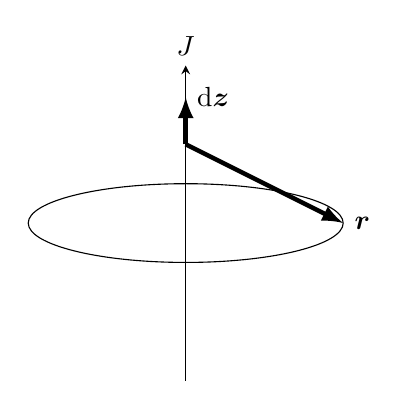
\begin{tikzpicture}
      \draw[-stealth](0,-2,0) -- (0,2,0) node[above]{$J$};
      \draw[-latex,ultra thick](0,1,0)--(0,1.6,0) node [right]{$\dd \bm{z}$};
      \draw[-latex,ultra thick](0,1,0)--(2,0,0) node [right]{$\bm{r}$};
      \draw[thin](0,0,0) circle [x radius=2, y radius=0.5];
    \end{tikzpicture}
    \caption{直線電流}
    \label{current}
  \end{figure}

\end{itemize}


\clearpage
\prb{5}{量子力学}
\begin{enumerate}
  \item 
  対角化されているので,固有値は$\varepsilon_{\text{L}},\varepsilon_{\text{R}}$で対応する固有ベクトルはそれぞれ$\ket{\text{L}},\ket{\text{R}}$.

  \item 
  非対角成分が$\Delta$なので
  \begin{equation}
    H
    =
    \begin{pmatrix}
      \varepsilon_{\text{L}}
      &
      \Delta 
      \\
      \Delta
      &
      \varepsilon_{\text{R}}
    \end{pmatrix}
  \end{equation}
  である.

  \item 
  固有方程式は
  \begin{equation}
    (\lambda-\varepsilon_{\text{L}})(\lambda-\varepsilon_{\text{R}})
    -
    \Delta^2
    =
    0
  \end{equation}
  であり,これを解くと
  \begin{equation}
    \lambda_{\pm}
    =
    \frac{\varepsilon_{\text{L}}+\varepsilon_{\text{R}}\pm\sqrt{(\varepsilon_{\text{L}}-\varepsilon_{\text{R}})^2+\Delta^2}}{2}
  \end{equation}
  である.

  \item
  固有値は
  \begin{equation}
    \lambda_{\pm}
    =
    \varepsilon
    \pm
    \Delta
    \label{eigen}
  \end{equation}
  である.これらに対応する固有ベクトルはそれぞれ
  \begin{equation}
    \frac{\ket{\text{L}}+\ket{\text{R}}}{\sqrt{2}}
    \ ,\ 
    \frac{\ket{\text{L}}-\ket{\text{R}}}{\sqrt{2}}
  \end{equation}
  である.

  \item 
  行列は
  \begin{equation}
    \hat{X}
    =
    \begin{pmatrix}
      1 & 0 \\
      0 & -1
    \end{pmatrix}
    \ ,\ 
    \hat{Y}
    =
    \begin{pmatrix}
      0 & 1 \\
      1 & 0
    \end{pmatrix}
  \end{equation}
  である.よって,
  \begin{equation}
    \hat{Z}
    =
    \begin{pmatrix}
      0 & i \\
      -i & 0
    \end{pmatrix}
    \ ,\ \ 
    \left[ \hat{Y},\hat{Z} \right]
    =
    \begin{pmatrix}
      -2i & 0 \\
      0 & 2i
    \end{pmatrix}
    \ ,\ \ 
    \left[ \hat{Z},\hat{X} \right]
    =
    \begin{pmatrix}
      0 & -2i \\
      -2i & 0
    \end{pmatrix}
  \end{equation}
  である.

  \item 
  $H^{n}$をもとめよう.対角化はできているの
  \begin{equation}
    \bm{v}_{1}
    =
    \frac{1}{\sqrt{2}}\begin{pmatrix}
      1 \\
      1
    \end{pmatrix}
    \ ,\ \bm{v}_{2}
    =
    \frac{1}{\sqrt{2}}\begin{pmatrix}
      1 \\
      -1
    \end{pmatrix}
  \end{equation}
  として$P=(\bm{v}_{1}\ \bm{v}_{2})$とすれば,その逆行列は
  \begin{equation}
    P^{-1}
    =
    \frac{1}{\sqrt{2}}
    \begin{pmatrix}
      1 & 1 \\
      1 & -1
    \end{pmatrix}
  \end{equation}
  である.したがって,
  \begin{equation}
    \begin{pmatrix}
      \varepsilon+\Delta & 0 \\
      0 & \varepsilon-\Delta
    \end{pmatrix}
    =
    P^{-1}
    H
    P
  \end{equation}
  なので,
  \begin{equation}
    H^{n}
    =
    P
    \begin{pmatrix}
      (\varepsilon+\Delta)^{n} & 0 \\
      0 & (\varepsilon-\Delta)^{n}
    \end{pmatrix}
    P^{-1}
    =
    \frac{1}{2}
    \begin{pmatrix}
      \lambda_{+}^{n}+\lambda_{-}^{n}
      &
      \lambda_{+}^{n}-\lambda_{-}^{n}
      \\
      \lambda_{+}^{n}-\lambda_{-}^{n}
      &
      \lambda_{+}^{n}+\lambda_{-}^{n}
    \end{pmatrix}
  \end{equation}
  である.ただし,表記は\eqref{eigen}を用いた.したがって,
  \begin{align}
    e^{-iHt/\hbar}
    &=
    \sum_{n=0}^{\infty}
    \frac{(-it/\hbar)^n}{n!}
    \cdot
    \frac{1}{2}
    \begin{pmatrix}
      \lambda_{+}^{n}+\lambda_{-}^{n}
      &
      \lambda_{+}^{n}-\lambda_{-}^{n}
      \\
      \lambda_{+}^{n}-\lambda_{-}^{n}
      &
      \lambda_{+}^{n}+\lambda_{-}^{n}
    \end{pmatrix}
    \nonumber
    \\
    &=
    \frac{1}{2}
    \begin{pmatrix}
      e^{-i\lambda_{+}t/\hbar}+e^{-i\lambda_{-}t/\hbar}
      &
      e^{-i\lambda_{+}t/\hbar}-e^{-i\lambda_{-}t/\hbar}
      \\
      e^{-i\lambda_{+}t/\hbar}-e^{-i\lambda_{-}t/\hbar}
      &
      e^{-i\lambda_{+}t/\hbar}+e^{-i\lambda_{-}t/\hbar}
    \end{pmatrix}
  \end{align}
  である.

  \item 
  計算すれば
  \begin{align*}
    e^{-iHt/\hbar}\ket{\psi(0)}
    &=
    \frac{1}{2}
    \begin{pmatrix}
      e^{-i\lambda_{+}t/\hbar}+e^{-i\lambda_{-}t/\hbar}
      &
      e^{-i\lambda_{+}t/\hbar}-e^{-i\lambda_{-}t/\hbar}
      \\
      e^{-i\lambda_{+}t/\hbar}-e^{-i\lambda_{-}t/\hbar}
      &
      e^{-i\lambda_{+}t/\hbar}+e^{-i\lambda_{-}t/\hbar}
    \end{pmatrix}
    \begin{pmatrix}
      1 \\
      0
    \end{pmatrix}
    \nonumber
    \\
    &=
    \frac{1}{2}
    \begin{pmatrix}
      e^{-i\lambda_{+}t/\hbar}+e^{-i\lambda_{-}t/\hbar}
      \\
      e^{-i\lambda_{+}t/\hbar}-e^{-i\lambda_{-}t/\hbar}
    \end{pmatrix}
  \end{align*}
  である.

  \item 
  \begin{align*}
    P_{L}(t)
    &=
    |\braket{\text{L}|\psi(t)}|^2
    \nonumber
    \\
    &=
    \frac{1}{4}\left[ 2+e^{+2i\Delta t/\hbar}+e^{-2i\Delta t/\hbar} \right]
    \nonumber
    \\
    &=
    \frac{1+\cos(2\Delta t/\hbar)}{2}
    \\
    P_{R}(t)
    &=
    |\braket{\text{R}|\psi(t)}|^2
    \nonumber
    \\
    &=
    \frac{1}{4}\left[ 2-e^{+2i\Delta t/\hbar}-e^{-2i\Delta t/\hbar} \right]
    \nonumber
    \\
    &=
    \frac{1-\cos(2\Delta t/\hbar)}{2}
  \end{align*}
  である\footnote{ちゃんと足すと$1$.}.

  \item 
  周期は$T=\pi\hbar/\Delta$で,中心は$P=1/2$であることに注意すれば,図\ref{PLPR}のようになる.

  \begin{figure}[ht]
    \centering    
    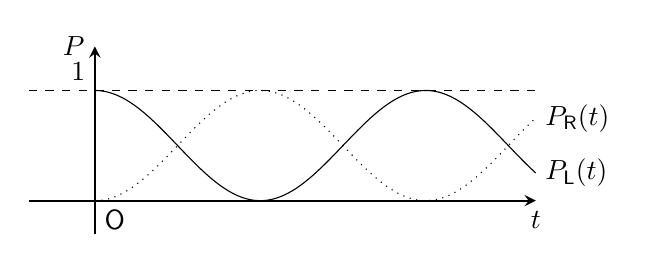
\begin{tikzpicture}[scale=1.4]
        \draw[->,>=stealth,thick](-0.6,0)--(4,0)node[below]{$t$};
        \draw[->,>=stealth,thick](0,-0.3)--(0,1.4)node[left]{$P$};
        \draw(0,0)node[below right]{O};
        \draw[dashed,thin](-0.6,1)--(4,1);
        \draw(0,1)node[above left]{$1$};
        \draw[samples=100,domain=0:4]plot(\x,{(1+cos(\x*360/3))/2})node[right]{$P_{\text{L}}(t)$};
        \draw[samples=100,domain=0:4,dotted]plot(\x,{(1-cos(\x*360/3))/2})node[right]{$P_{\text{R}}(t)$};
      \end{tikzpicture}    
      \caption{$P_{\text{L}}$と$P_{{\text{R}}}$の時間変化}
      \label{PLPR}
  \end{figure}

\end{enumerate}

\clearpage
\prb{6}{統計力学}
\begin{enumerate}
  \item 
  問題文から,自由度が7であることがわかり,それぞれにエネルギーが等分配されるので
  \begin{equation}
    U
    =
    \frac{7}{2}Nk_{B}T
  \end{equation}
  である.

  \item   
  定義から
  \begin{equation}
    C_{V}
    =
    \pdv{U}{T}
    =
    \frac{7}{2}Nk_{B}
    \ .
  \end{equation}

  \item 
  ハミルトニアンが
  \begin{equation}
    H
    =
    H_{\text{CM}}
    +
    H_{\text{rel}}
  \end{equation}
  と分離できていれば
  \begin{equation}
    Z
    =
    \sum_{\sigma}e^{-\beta(H_{\text{CM}}
    +
    H_{\text{rel}})}
    =
    \sum_{\sigma_{\text{CM}}}e^{-\beta H_{\text{CM}}}
    \sum_{\sigma_{\text{rel}}}e^{-\beta H_{\text{rel}}}
    =
    z_{\text{CM}}^{N}z_{\text{rel}}^{N}
  \end{equation}
  である.

  \item 
  全体の分配関数は
  \begin{equation}
    Z
    =
    V^{N}\left( \frac{M}{2\pi\hbar^2 \beta} \right)^{3N/2}z_{\text{rel}}^{N}
  \end{equation}
  であり,
  \begin{equation}
    F
    =
    -\frac{1}{\beta}\log Z
    =
    -\frac{N\log V}{\beta}+(\text{$V$に関係ない項})
  \end{equation}
  なので,
  \begin{equation}
    p
    =
    -\pdv{F}{V}
    =
    \frac{N}{\beta V}
    =
    \frac{Nk_{B}T}{V}
  \end{equation}
  である.よって,状態方程式は
  \begin{equation}
    pV
    =
    Nk_{B}T
  \end{equation}
  である.

  \item 
  $\theta,\varphi,r$はそれぞれ別に積分できて
  \begin{equation}
    \int_{0}^{\pi}\dd \theta\ \sin\theta
    =
    2
    \ ,\ 
    \int_{0}^{2\pi}
    \dd \varphi
    =
    2\pi
    \ ,\ 
    \int_{-\infty}^{\infty}\dd r\ 
    \exp\left[ -\frac{\beta}{2}m\omega^2(r-a)^2 \right]
    =
    \sqrt{\frac{2\pi}{\beta m\omega^2}}
  \end{equation}
  なので
  \begin{equation}
    z_{\text{rel}}
    =
    \frac{2ma^2}{\hbar^3 \beta^2 \omega}
  \end{equation}
  である.

  \item   
  分配関数は
  \begin{equation}
    Z
    =
    V^{N}\left( \frac{M}{2\pi\hbar^2 \beta} \right)^{3N/2}
    \cdot
    \left(  
      \frac{2ma^2}{\hbar^3 \beta^2 \omega}
    \right)^{N}
  \end{equation}
  である.よって,
  \begin{align}
    U
    &=
    F+TS
    \nonumber
    \\
    &=
    F
    -
    T\pdv{F}{T}
  \end{align}
  より,
  \begin{equation}
    F
    =
    -\frac{7}{2}Nk_{B}T\log T
    +
    (\text{$T$に関係ない項})
  \end{equation}
  なので,
  \begin{equation}
    U
    =
    \frac{7}{2}Nk_{B}T
    +
    (\text{$T$に関係ない項})
  \end{equation}
  である.これを$T$で微分すれば
  \begin{equation}
    C
    =
    \pdv{U}{V}
    =
    \frac{7}{2}Nk_{B}
  \end{equation}
  と(1),(2)と同じ結果になる.

  \item 
  それぞれ
  \begin{equation}
    z_{\text{vib}}(\beta)
    =
    \sum_{n=0}^{\infty}\exp\left[ -\beta \hbar\omega\left( n+\frac{1}{2} \right) \right]
    \ ,\ 
    z_{\text{rot}}(\beta)
    =
    \sum_{l=0}^{\infty}(2l+1)\exp\left[ -\beta \frac{\hbar^2 l(l+1)}{2ma^2} \right]
  \end{equation}
  である\footnote{$z_{\text{vib}}$のほうは,無限等比級数でもうちょっと計算できますが,問題文にあったのでたぶんこれでOK.}\footnote{$2l+1$重に縮退しているので,そこはちゃんと足さないといけません.}.

  \item 
  室温では
  \begin{equation}
    \frac{\hbar^2 \beta}{2ma^2}
    \ll
    1
    \ll
    \beta\hbar\omega
  \end{equation}  
  である.ここで,$z_{\text{vib}}$を計算して$\beta\hbar\omega\gg 1$で近似すると
  \begin{equation}
    z_{\text{vib}}
    =
    \frac{1}{e^{\beta\hbar\omega/2}-e^{-\beta\hbar\omega/2}}
    \sim
    e^{-\beta\hbar\omega/2}
  \end{equation}
  である.したがって,振動のエネルギーは
  \begin{equation}
    U_{\text{vib}}
    =
    -\pdv{}{\beta}N\log z_{\text{vib}}
    =
    \frac{N\hbar\omega}{2}
  \end{equation}
  であり,振動による比熱への寄与は$0$である.回転の分配関数は,
  \begin{equation}
    f(x)
    =
    (2x+1)\exp\left[ -\sigma x(x+1) \right]
    \ ,\ 
    \sigma
    =
    \frac{\beta\hbar^2}{2ma^2}
  \end{equation}
  とおけば\eqref{EulerMac}が使えて$f(0)=1,f'(0)=2-\sigma$であり\footnote{
    $f'(x)$は
    \begin{equation}
      f'(x)
      =
      \left\{  
        2-\sigma(2x+1)^{2}
      \right\}
      e^{-\sigma x(x+1)}
    \end{equation}
    です.
  },
  \begin{equation}
    \int_{0}^{\infty}f(x)\dd x
    =
    \frac{1}{\sigma}\int_{0}^{\infty}e^{-\sigma x(x+1)}(\sigma x(x+1))' \dd x
    =
    \frac{1}{\sigma}\int_{0}^{\infty} e^{-\xi} \dd \xi
    =
    \frac{1}{\sigma}
  \end{equation}
  なので,
  \begin{equation}
    z_{\text{rot}}
    =
    \frac{5}{2}
    +
    \frac{2ma^2}{\beta\hbar^2}
    -
    \mathcal{O}(\sigma)
    =
    \frac{2ma^2}{\beta\hbar^2}
    \left\{  
      1+\frac{5}{2}\cdot\frac{\beta\hbar^2}{2ma^2}
      +
      \mathcal{O}(\sigma^2)
    \right\}
    \sim
    \frac{2ma^2}{\beta\hbar^2}
    \label{part_rot}
  \end{equation}
  である.よって
  \begin{equation}
    U_{\text{rot}}
    =
    -N\pdv{}{\beta}\log z_{\text{rot}}
    =
    Nk_{B}T
  \end{equation}
  であり,
  \begin{equation}
    C
    =
    \pdv{U}{T}
    =
    Nk_{B}
  \end{equation}
  となる.

\end{enumerate}

\subsection*{補足}
\begin{itemize}
  \item 
  設問(8)の計算はオイラー・マクローリンの公式と言うらしいです.関数$f(x)$が$C^{\infty}$級なら
  \begin{equation}
    \sum_{n=0}^{\infty}f(n)
    =
    \int_{0}^{\infty}f(x)\dd x
    +
    \frac{1}{2}f(0)
    +
    -\frac{1}{12}f'(0)
    +
    \cdots
    \label{EulerMac}
  \end{equation}
  という等式が成立するそう.今回は,この近似の1次を拾ってくるだけでよさそうなかんじ.試験中はあまりこういった公式にとらわれず,えいやっと積分に書き換えちゃうのが現実的な気がします.

  \item 
  実は,\eqref{part_rot}は古典近似と一致します\footnote{
    つまり,近似で落とした項が量子論からの寄与です.
  }.古典論からの系のハミルトニアンは
  \begin{equation}
    H
    =
    \frac{1}{2I}p_{\theta}^2
    +
    \frac{1}{2I\sin^2\theta}p_{\varphi}^2
  \end{equation}
  と書けるので\footnote{
    ここで,$I$は慣性モーメントで
    \begin{equation}
      I
      =
      ma^2
    \end{equation}
    に対応します.
  },このときの分配関数は
  \begin{equation}
    z_{\text{rot}}
    =
    \frac{1}{h^2}
    \int_{0}^{\pi}\dd \theta\int_{0}^{2\pi}\dd\varphi
    \int_{-\infty}^{\infty}\dd p_{\theta}\int_{-\infty}^{\infty}\dd p_{\varphi}
    \exp\left[ -\frac{1}{k_{B}T}\left( \frac{1}{2I}p_{\theta}^2
    +
    \frac{1}{2I\sin^2\theta}p_{\varphi}^2 \right) \right]
  \end{equation}
  であり,これをちゃんと計算すると
  \begin{equation}
    z_{\text{rot}}
    =
    \frac{2Ik_{B}T}{\hbar^2}
  \end{equation}
  となって,確かに\eqref{part_rot}と一致します.

\end{itemize}



\end{document}
